
\titleformat{\section}[hang]{\bfseries\huge}{}{0ex}{}[]
\input{../out/tex/00.2-Vorwort.tex}
\titleformat{\section}[wrap]{\bfseries\huge}{}{0ex}{}[]
\newpage

\tableofcontents
\newpage

\null\vfill
\begin{center}
\begin{minipage}[c]{\textwidth}
  \begin{center}
  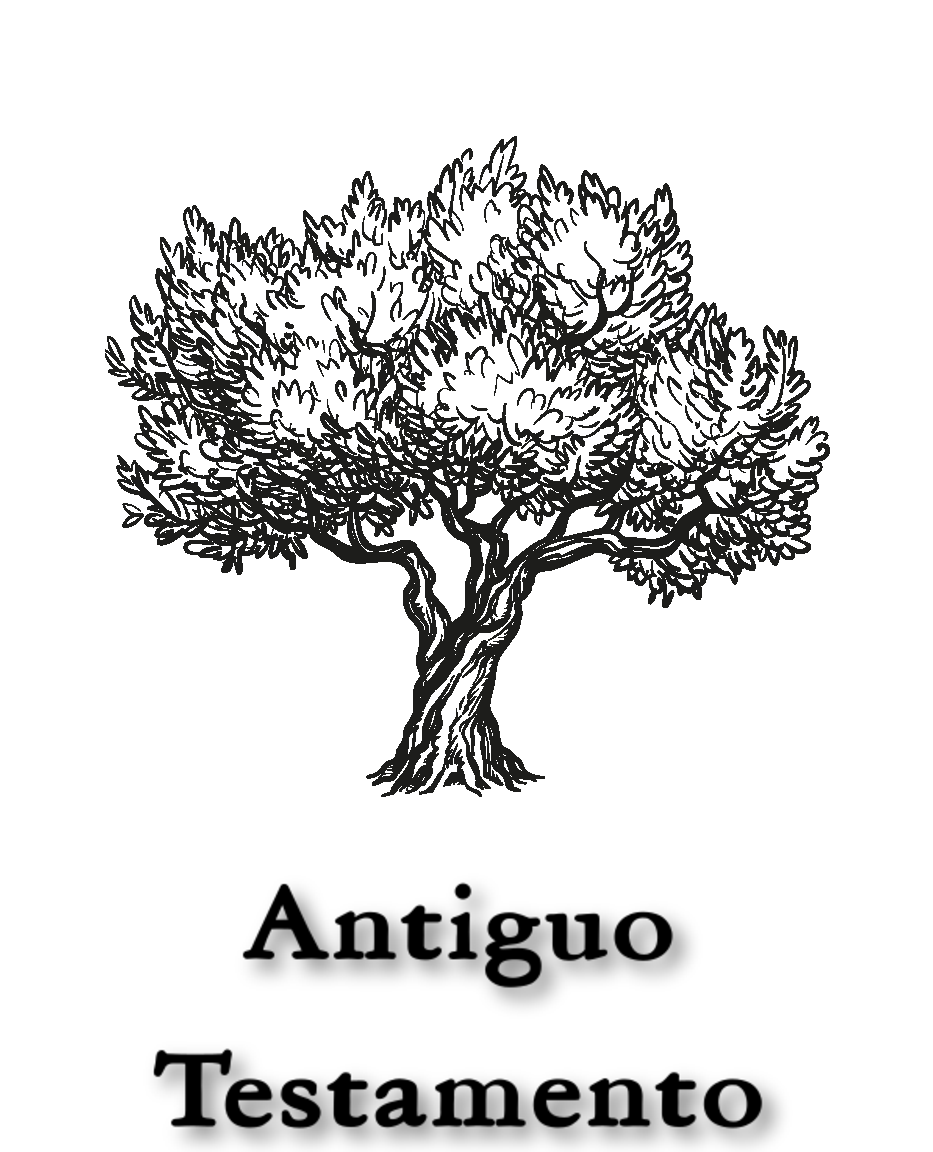
\includegraphics{AntiguoTestamentoTitulo.pdf}
  \end{center}
\end{minipage}
\end{center}
\null\vfill
\newpage

\pagestyle{bible}

\renewcommand{\cleardoublepage}{\clearpage}
%\renewcommand{\clearpage}{}

\chapter{Das erste Buch Mose (Genesis)}
\begin{multicols}{2}
  \raggedcolumns
  \parskip=0pt \relax
  \input{../out/tex/01-1. Mose.tex}
\end{multicols}

\chapter{Das zweite Buch Mose (Exodus)}
\begin{multicols}{2}
  \raggedcolumns
  \parskip=0pt \relax
  \input{../out/tex/02-2. Mose.tex}
\end{multicols}

\chapter{Das dritte Buch Mose (Leviticus)}
\begin{multicols}{2}
  \raggedcolumns
  \parskip=0pt \relax
  \input{../out/tex/03-3. Mose.tex}
\end{multicols}

\chapter{Das vierte Buch Mose (Numeri)}
\begin{multicols}{2}
  \raggedcolumns
  \parskip=0pt \relax
  \input{../out/tex/04-4. Mose.tex}
\end{multicols}

\chapter{Das fünfte Buch Mose (Deuteronomium)}
\begin{multicols}{2}
  \raggedcolumns
  \parskip=0pt \relax
  \input{../out/tex/05-5. Mose.tex}
\end{multicols}

\chapter{Josua}
\begin{multicols}{2}
  \raggedcolumns
  \parskip=0pt \relax
  \input{../out/tex/06-Josua.tex}
\end{multicols}

\chapter{Richter}
\begin{multicols}{2}
  \raggedcolumns
  \parskip=0pt \relax
  \input{../out/tex/07-Richter.tex}
\end{multicols}

\chapter{Ruth}
\begin{multicols}{2}
  \raggedcolumns
  \parskip=0pt \relax
  \input{../out/tex/08-Ruth.tex}
\end{multicols}

\chapter{1. Samuel}
\begin{multicols}{2}
  \raggedcolumns
  \parskip=0pt \relax
  \input{../out/tex/09-1. Samuel.tex}
\end{multicols}

\chapter{2. Samuel}
\begin{multicols}{2}
  \raggedcolumns
  \parskip=0pt \relax
  \input{../out/tex/10-2. Samuel.tex}
\end{multicols}

\chapter{1. Könige}
\begin{multicols}{2}
  \raggedcolumns
  \parskip=0pt \relax
  \input{../out/tex/11-1. Könige.tex}
\end{multicols}

\chapter{2. Könige}
\begin{multicols}{2}
  \raggedcolumns
  \parskip=0pt \relax
  \input{../out/tex/12-2. Könige.tex}
\end{multicols}

\chapter{1. Chronik}
\begin{multicols}{2}
  \raggedcolumns
  \parskip=0pt \relax
  \input{../out/tex/13-1. Chronik.tex}
\end{multicols}

\chapter{2. Chronik}
\begin{multicols}{2}
  \raggedcolumns
  \parskip=0pt \relax
  \input{../out/tex/14-2. Chronik.tex}
\end{multicols}

\chapter{Esra}
\begin{multicols}{2}
  \raggedcolumns
  \parskip=0pt \relax
  \input{../out/tex/15-Esra.tex}
\end{multicols}

\chapter{Nehemia}
\begin{multicols}{2}
  \raggedcolumns
  \parskip=0pt \relax
  \input{../out/tex/16-Nehemia.tex}
\end{multicols}

\chapter{Esther}
\begin{multicols}{2}
  \raggedcolumns
  \parskip=0pt \relax
  \input{../out/tex/17-Esther.tex}
\end{multicols}

\chapter{Hiob}
\begin{multicols}{2}
  \raggedcolumns
  \parskip=0pt \relax
  \input{../out/tex/18-Hiob.tex}
\end{multicols}

\chapter{Psalmen}
\begin{multicols}{2}
  \raggedcolumns
  \parskip=0pt \relax
  \input{../out/tex/19-Psalmen.tex}
\end{multicols}

\chapter{Sprüche}
\begin{multicols}{2}
  \raggedcolumns
  \parskip=0pt \relax
  \input{../out/tex/20-Sprüche.tex}
\end{multicols}

\chapter{Prediger}
\begin{multicols}{2}
  \raggedcolumns
  \parskip=0pt \relax
  \input{../out/tex/21-Prediger.tex}
\end{multicols}

\chapter{Hohelied}
\begin{multicols}{2}
  \raggedcolumns
  \parskip=0pt \relax
  \input{../out/tex/22-Hohelied.tex}
\end{multicols}

\chapter{Jesaia}
\begin{multicols}{2}
  \raggedcolumns
  \parskip=0pt \relax
  \input{../out/tex/23-Jesaja.tex}
\end{multicols}

\chapter{Jeremia}
\begin{multicols}{2}
  \raggedcolumns
  \parskip=0pt \relax
  \input{../out/tex/24-Jeremia.tex}
\end{multicols}

\chapter{Klagelieder}
\begin{multicols}{2}
  \raggedcolumns
  \parskip=0pt \relax
  \input{../out/tex/25-Klagelieder.tex}
\end{multicols}

\chapter{Hesekiel}
\begin{multicols}{2}
  \raggedcolumns
  \parskip=0pt \relax
  \input{../out/tex/26-Hesekiel.tex}
\end{multicols}

\chapter{Daniel}
\begin{multicols}{2}
  \raggedcolumns
  \parskip=0pt \relax
  \input{../out/tex/27-Daniel.tex}
\end{multicols}

\chapter{Hosea}
\begin{multicols}{2}
  \raggedcolumns
  \parskip=0pt \relax
  \input{../out/tex/28-Hosea.tex}
\end{multicols}

\chapter{Joel}
\begin{multicols}{2}
  \raggedcolumns
  \parskip=0pt \relax
  \input{../out/tex/29-Joel.tex}
\end{multicols}

\chapter{Amos}
\begin{multicols}{2}
  \raggedcolumns
  \parskip=0pt \relax
  \input{../out/tex/30-Amos.tex}
\end{multicols}

\chapter{Obadja}
\begin{multicols}{2}
  \raggedcolumns
  \parskip=0pt \relax
  \input{../out/tex/31-Obadja.tex}
\end{multicols}

\chapter{Jona}
\begin{multicols}{2}
  \raggedcolumns
  \parskip=0pt \relax
  \input{../out/tex/32-Jona.tex}
\end{multicols}

\chapter{Micha}
\begin{multicols}{2}
  \raggedcolumns
  \parskip=0pt \relax
  \input{../out/tex/33-Micha.tex}
\end{multicols}

\chapter{Nahum}
\begin{multicols}{2}
  \raggedcolumns
  \parskip=0pt \relax
  \input{../out/tex/34-Nahum.tex}
\end{multicols}

\chapter{Habakuk}
\begin{multicols}{2}
  \raggedcolumns
  \parskip=0pt \relax
  \input{../out/tex/35-Habakuk.tex}
\end{multicols}

\chapter{Zephanja}
\begin{multicols}{2}
  \raggedcolumns
  \parskip=0pt \relax
  \input{../out/tex/36-Zephanja.tex}
\end{multicols}

\chapter{Haggai}
\begin{multicols}{2}
  \raggedcolumns
  \parskip=0pt \relax
  \input{../out/tex/37-Haggai.tex}
\end{multicols}

\chapter{Sacharja}
\begin{multicols}{2}
  \raggedcolumns
  \parskip=0pt \relax
  \input{../out/tex/38-Sacharja.tex}
\end{multicols}

\chapter{Maleachi}
\begin{multicols}{2}
  \raggedcolumns
  \parskip=0pt \relax
  \input{../out/tex/39-Maleachi.tex}
\end{multicols}

\newpage

\pagestyle{empty}

\null\vfill
\begin{center}
\begin{minipage}[c]{\textwidth}
  \begin{center}
  
\includegraphics{NuevoTestamentoTitulo.pdf}
  \end{center}
\end{minipage}
\end{center}
\null\vfill
\newpage

\pagestyle{bible}

\chapter{Matthäus}
\begin{multicols}{2}
  \raggedcolumns
  \parskip=0pt \relax
  \input{../out/tex/40-Matthäus.tex}
\end{multicols}

\chapter{Markus}
\begin{multicols}{2}
  \raggedcolumns
  \parskip=0pt \relax
  \input{../out/tex/41-Markus.tex}
\end{multicols}

\chapter{Lukas}
\begin{multicols}{2}
  \raggedcolumns
  \parskip=0pt \relax
  \input{../out/tex/42-Lukas.tex}
\end{multicols}

\chapter{Johannes}
\begin{multicols}{2}
  \raggedcolumns
  \parskip=0pt \relax
  \input{../out/tex/43-Johannes.tex}
\end{multicols}

\chapter{Apostelgeschichte}
\begin{multicols}{2}
  \raggedcolumns
  \parskip=0pt \relax
  \input{../out/tex/44-Apostelgeschichte.tex}
\end{multicols}

\chapter{Römer}
\begin{multicols}{2}
  \raggedcolumns
  \parskip=0pt \relax
  \input{../out/tex/45-Römer.tex}
\end{multicols}

\chapter{1. Korinther}
\begin{multicols}{2}
  \raggedcolumns
  \parskip=0pt \relax
  \input{../out/tex/46-1. Korinther.tex}
\end{multicols}

\chapter{2. Korinther}
\begin{multicols}{2}
  \raggedcolumns
  \parskip=0pt \relax
  \input{../out/tex/47-2. Korinther.tex}
\end{multicols}

\chapter{Galater}
\begin{multicols}{2}
  \raggedcolumns
  \parskip=0pt \relax
  \input{../out/tex/48-Galater.tex}
\end{multicols}

\chapter{Epheser}
\begin{multicols}{2}
  \raggedcolumns
  \parskip=0pt \relax
  \input{../out/tex/49-Epheser.tex}
\end{multicols}

\chapter{Philipper}
\begin{multicols}{2}
  \raggedcolumns
  \parskip=0pt \relax
  \input{../out/tex/50-Philipper.tex}
\end{multicols}

\chapter{Kolosser}
\begin{multicols}{2}
  \raggedcolumns
  \parskip=0pt \relax
  \input{../out/tex/51-Kolosser.tex}
\end{multicols}

\chapter{1. Thessalonicher}
\begin{multicols}{2}
  \raggedcolumns
  \parskip=0pt \relax
  \input{../out/tex/52-1. Thessalonicher.tex}
\end{multicols}

\chapter{2. Thessalonicher}
\begin{multicols}{2}
  \raggedcolumns
  \parskip=0pt \relax
  \input{../out/tex/53-2. Thessalonicher.tex}
\end{multicols}

\chapter{1. Timotheus}
\begin{multicols}{2}
  \raggedcolumns
  \parskip=0pt \relax
  \input{../out/tex/54-1. Timotheus.tex}
\end{multicols}

\chapter{2. Timotheus}
\begin{multicols}{2}
  \raggedcolumns
  \parskip=0pt \relax
  \input{../out/tex/55-2. Timotheus.tex}
\end{multicols}

\chapter{Titus}
\begin{multicols}{2}
  \raggedcolumns
  \parskip=0pt \relax
  \input{../out/tex/56-Titus.tex}
\end{multicols}

\chapter{Philemon}
\begin{multicols}{2}
  \raggedcolumns
  \parskip=0pt \relax
  \input{../out/tex/57-Philemon.tex}
\end{multicols}

\chapter{Hebräer}
\begin{multicols}{2}
  \raggedcolumns
  \parskip=0pt \relax
  \input{../out/tex/58-Hebräer.tex}
\end{multicols}

\chapter{Jakobus}
\begin{multicols}{2}
  \raggedcolumns
  \parskip=0pt \relax
  \input{../out/tex/59-Jakobus.tex}
\end{multicols}

\chapter{1. Petrus}
\begin{multicols}{2}
  \raggedcolumns
  \parskip=0pt \relax
  \input{../out/tex/60-1. Petrus.tex}
\end{multicols}

\chapter{2 Petrus}
\begin{multicols}{2}
  \raggedcolumns
  \parskip=0pt \relax
  \input{../out/tex/61-2. Petrus.tex}
\end{multicols}

\chapter{1. Johannes}
\begin{multicols}{2}
  \raggedcolumns
  \parskip=0pt \relax
  \input{../out/tex/62-1. Johannes.tex}
\end{multicols}

\chapter{2. Johannes}
\begin{multicols}{2}
  \raggedcolumns
  \parskip=0pt \relax
  \input{../out/tex/63-2. Johannes.tex}
\end{multicols}

\chapter{3. Johannes}
\begin{multicols}{2}
  \raggedcolumns
  \parskip=0pt \relax
  \input{../out/tex/64-3. Johannes.tex}
\end{multicols}

\chapter{Judas}
\begin{multicols}{2}
  \raggedcolumns
  \parskip=0pt \relax
  \input{../out/tex/65-Judas.tex}
\end{multicols}

\chapter{Offenbarung}
\begin{multicols}{2}
  \raggedcolumns
  \parskip=0pt \relax
  \input{../out/tex/66-Offenbarung.tex}
\end{multicols}
\newpage

\end{document}



















